\documentclass[12pt]{article}
\usepackage{amsmath}
\usepackage{amsfonts}
\usepackage{enumerate}
\usepackage{pgfplots}
\usepackage{calc}
\usepackage{graphicx}
\usepackage{float}
\usepackage{hyperref}
\usepackage{chngpage}
\pgfplotsset{compat=1.12}
\hypersetup{colorlinks,urlcolor=blue}
\graphicspath{{./code/src/}}
\begin{document}
\title{Computer Science M146, Homework 1}
\date{January 30th, 2018}
\author{Michael Wu\\UID: 404751542}
\maketitle

\section*{Problem 1}

\paragraph{a)}

The best \(1\)-leaf decision tree will always predict \(1\). This is wrong \(\frac{1}{8}\) of the time. Thus over \(2^n\) training examples
the decision tree will make \(2^{n-3}\) mistakes.

\paragraph{b)}

No, because if we were to split based on any one of \(X_i\), we would predict \(1\) when \(X_i=1\) and when \(X_i=0\). This is because any split
on any variable yields a majority of results \(Y=1\) on either branch of the tree. This results in the exact same configuration as the \(1\)-leaf
decision tree.

\paragraph{c)}

\[E(Y)=-\frac{1}{8}\log_2\left(\frac{1}{8}\right)-\frac{7}{8}\log_2\left(\frac{7}{8}\right)\approx 0.5436\]

\paragraph{d)}

Yes. Splitting by any one of \(X_1,X_2,X_3\) yields entropy

\begin{align*}
        E(Y)&=\frac{1}{2}(-1\log(1))+\frac{1}{2}\left(-\frac{1}{4}\log_2\left(\frac{1}{4}\right)-\frac{3}{4}\log_2\left(\frac{3}{4}\right)\right)\\
        &=0+\frac{1}{2}\left(-\frac{1}{4}\log_2\left(\frac{1}{4}\right)-\frac{3}{4}\log_2\left(\frac{3}{4}\right)\right)\\
        &\approx 0.4056
\end{align*}

\section*{Problem 2}

\paragraph{a)}

Let \(C=\frac{p_k}{p_k+n_k}\) be a constant. Then the number of positive examples \(p\) is given by
\[p=\sum_{\forall k} C|S_k|=C|S|\]
Because \(|S|=p+n\), we know that the proportion of positive examples \(\frac{p}{p+n}\) is equal to \(C\). The proportion
of negative examples is the complement of this, \(1-C\). Additionally, we are given that the proportion of negative
and positive examples is also the same for every subset \(S_k\). Thus we calculate the entropy for the entire set \(S\)
\[E(S)=B(C)=-C\log_2(C)-(1-C)\log_2(1-C)\]
We then calculate the conditional entropy based on our split by attribute \(X_j\).
\[E_{X_j}(S)=\sum_{\forall k} \frac{|S_k|}{|S|} B(C)=\frac{|S|}{|S|}B(C)=-C\log_2(C)-(1-C)\log_2(1-C)\]
Our information gain is thus the difference between \(E(S)\) and \(E_{X_j}(S)\), which is zero.

\section*{Problem 3}

\paragraph{a)}

Because data points are their own closest neighbor, a value of \(k=1\) will always predict the correct value for the training data.
The resulting training error is \(0\%\).

\paragraph{b)}

Using too large values of \(k\) will be bad for this dataset due to underfitting. The two positives and the two negatives on the top left
and bottom right, respectively, would be drowned out by the other data points near them for \(k>3\). They would have no effect on the prediction,
which may lead to an inaccurate model. Eventually if \(k\) is big enough, points on the opposite side of the graph would affect predictions, which makes little sense.
In contrast a too small value of \(k\) may lead to overfitting, so if the stray negatives and positives were just noise, the model
may make the wrong prediction based on the noise. Predictions won't be averaged out like it would with higher \(k\).

\paragraph{c)}

A value of \(k=5\) minimizes leave-one-out cross validation error. There would be \(14\) different training and validation cases, of which
two positives in the top left and two negatives in the bottom right would be wrong. This leads to a training error of
\[\frac{4}{14}\approx 28.57\%\]

\section*{Problem 4.1}

\paragraph{a)}

For \texttt{Pclass}, I noticed that \(1\)st class and \(2\)nd class passengers
had a much higher rate of survival than \(3\)rd class passengers. There are many
more passengers in \(3\)rd class than in \(1\)st or \(2\)nd. For \texttt{Sex},
I noticed that women had a  higher chance of survival than men. For \texttt{Age}, it
appears that most children under \(10\) survived, and the elderly and young survive
more than people in their twenties and thirties. For \texttt{SibSp}, having between
one and three siblings and spouses ensured a higher rate of survival. For
\texttt{Parch}, having more parents and children ensured higher rates of survival.
For \texttt{Fare}, more expensive fares ensured a higher rate of survival. For
\texttt{Embarked}, it appears that people from Cherbourg had the highest rate of
survival, then Southampton and Queenstown had a similar rate of survival. Most
passengers embarked at Southampton. \texttt{Age}, \texttt{SibSp}, \texttt{Parch},
and \texttt{Fare} all show positive skews.

\begin{figure}[H]
        \begin{adjustwidth}{-10in}{-10in}
                \begin{center}
                        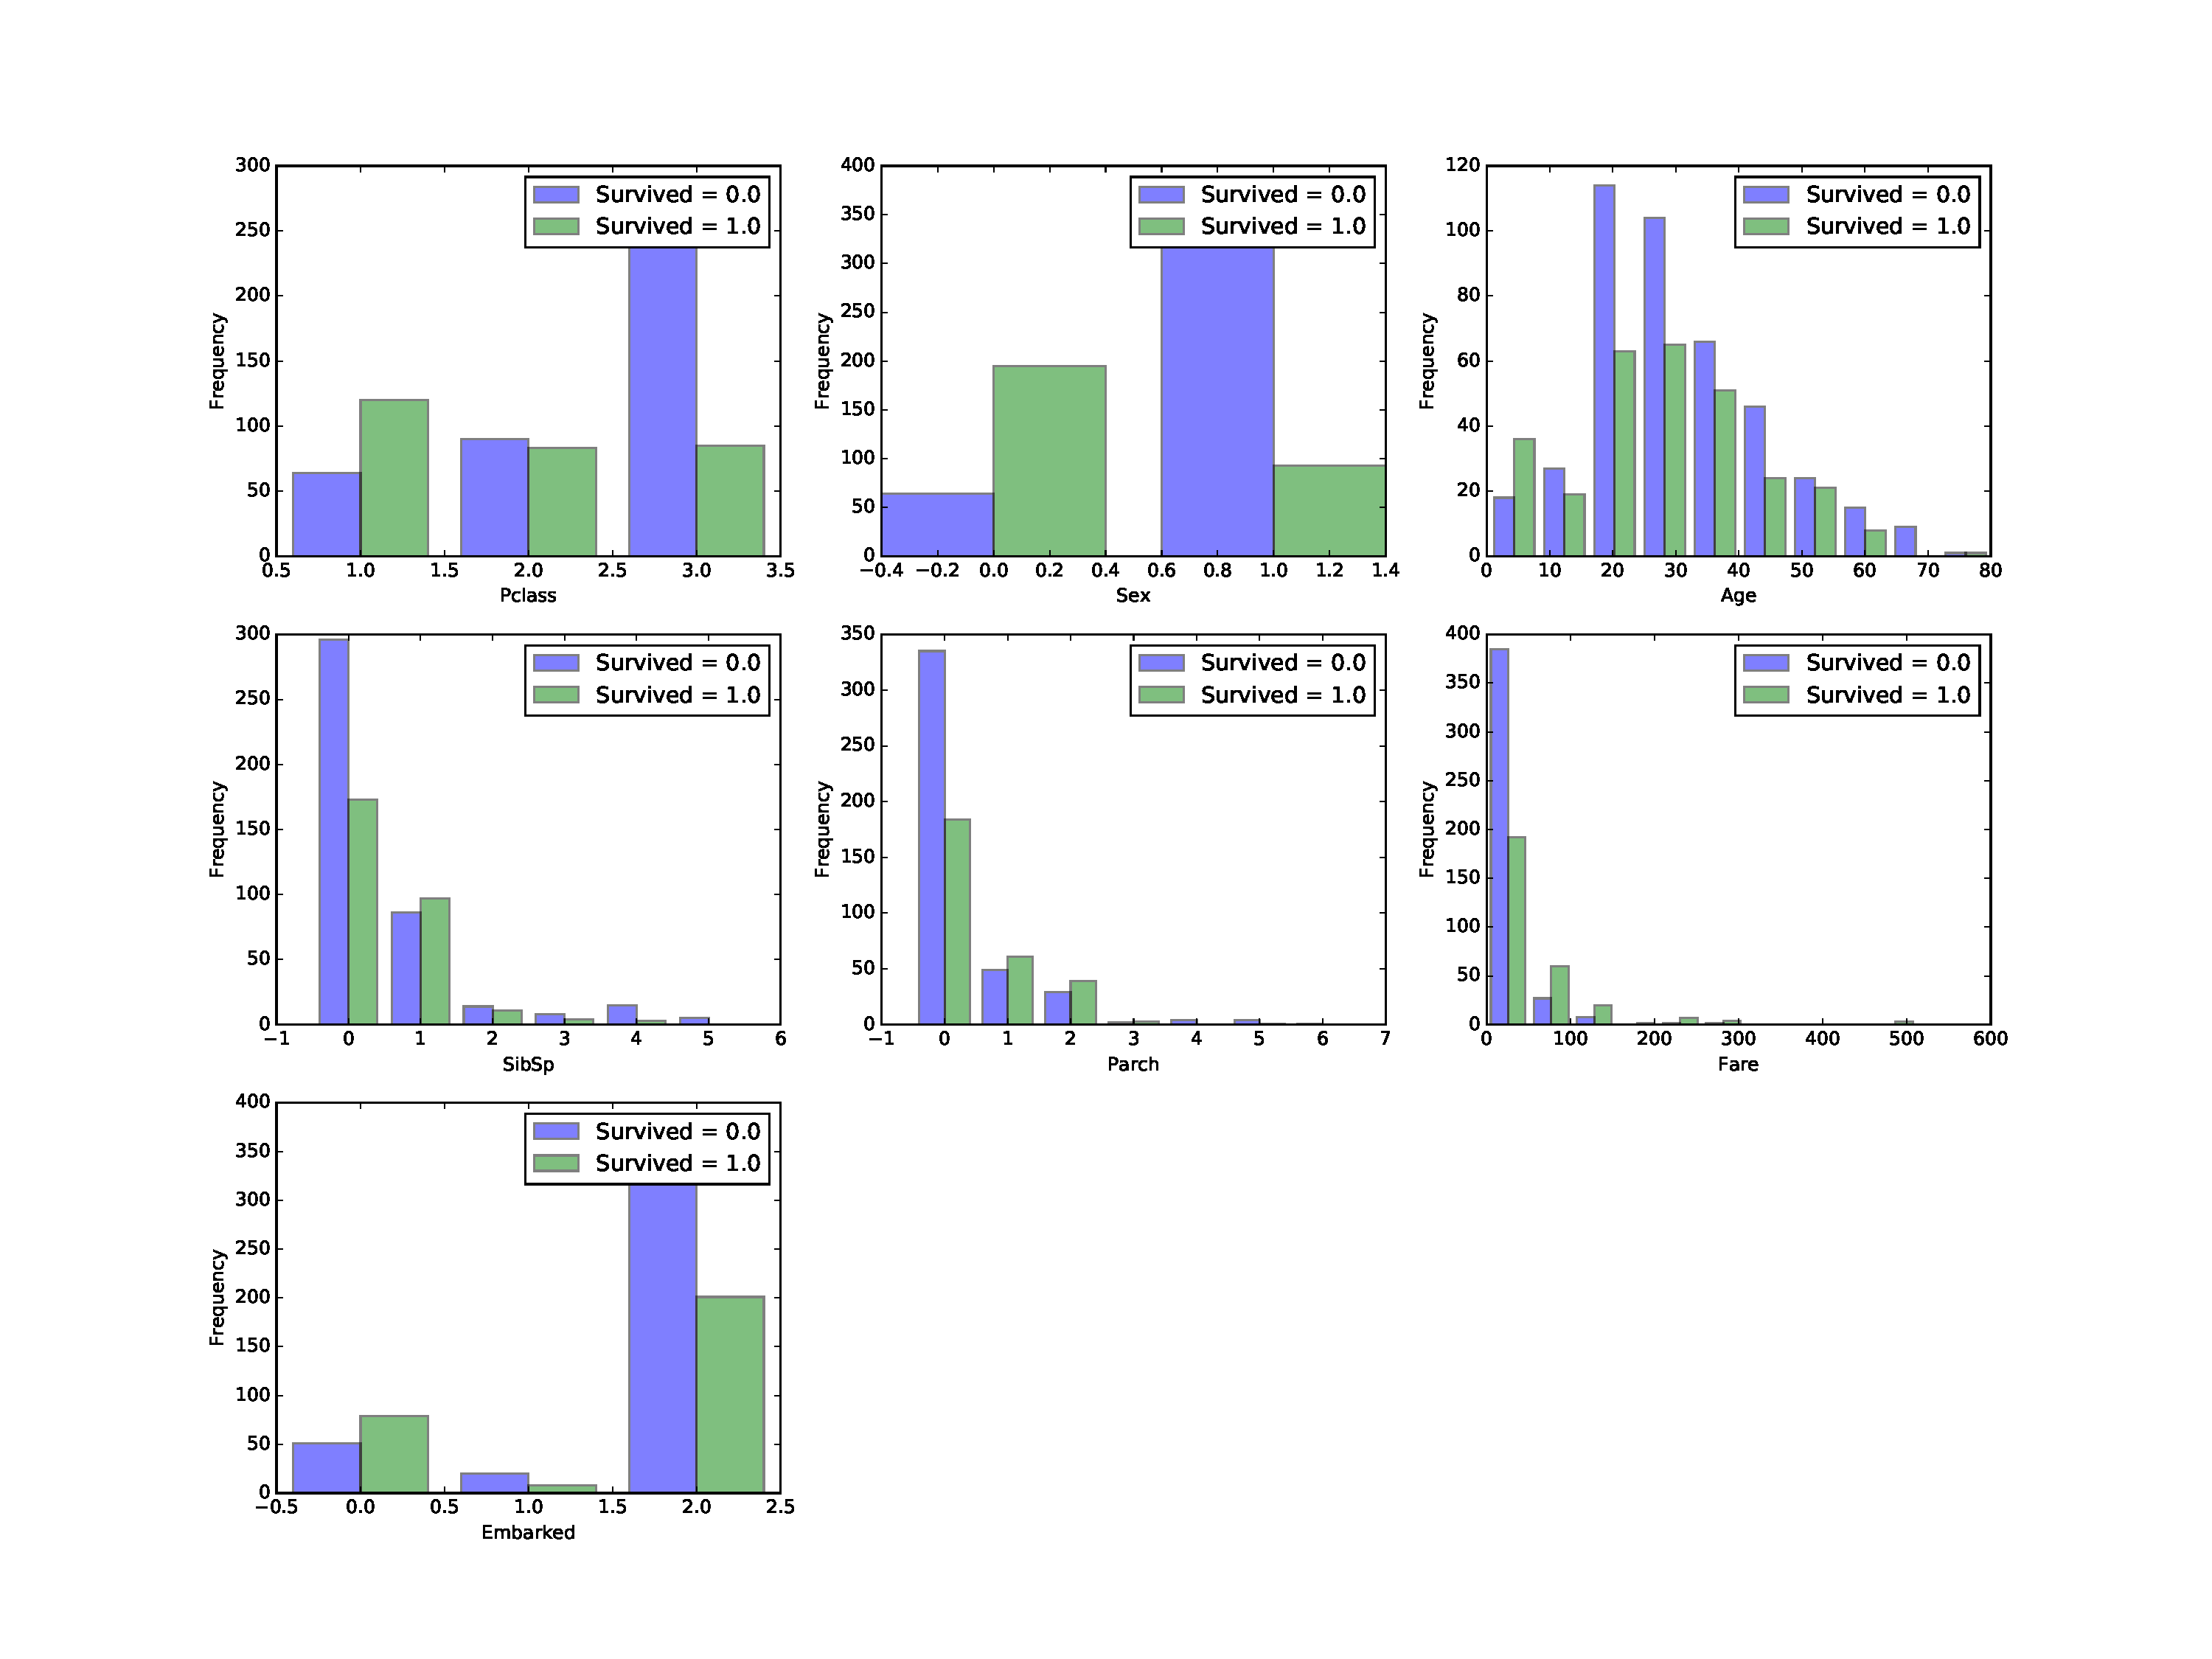
\includegraphics[width=8.5in,height=\textheight,keepaspectratio]{histograms}
                        \caption{Generated histograms from \texttt{titanic\_train.csv} for problem 4.1.}
                \end{center}
        \end{adjustwidth}
\end{figure}

\section*{Problem 4.2}

\paragraph{b)}

My implementation of the \texttt{RandomClassifier} class included the following methods.

\begin{verbatim}
def fit(self, X, y) :
    self.probabilities_ = {}

    for i in y.flat:
        if i in self.probabilities_:
            self.probabilities_[i]=self.probabilities_[i]+1
        else:
            self.probabilities_[i]=1

    for i in self.probabilities_.keys():
        self.probabilities_[i]= \
            self.probabilities_[i]/float(y.size)

    return self

def predict(self, X, seed=1234) :
    if self.probabilities_ is None :
        raise Exception("Classifier not initialized.",\
                "Perform a fit first.")
    np.random.seed(seed)

    n,d = X.shape
    y = np.random.choice(self.probabilities_.keys(),
        n, p=self.probabilities_.values())

    return y
\end{verbatim}

This gave me the expected training error of \(0.485\).

\paragraph{c)}

The training error of the \texttt{DecisionTreeClassifier} was \(0.014\).

\paragraph{d)}

The training error of the \texttt{KNeighborsClassifier} was \(0.162\) for \(K=3\), \(0.201\) for \(K=5\), and \(0.240\) for \(K=7\).

\paragraph{e)}

The errors are shown in the following table.\\

\begin{center}
        \begin{tabular}{c | c c}
                Classifier & Training Error & Testing Error\\
                \hline
                MajorityVote & 0.404 & 0.407\\
                Random & 0.489 & 0.487\\
                DecisionTree & 0.012 & 0.241\\
                5-NN & 0.212 & 0.315
        \end{tabular}
\end{center}

\paragraph{f)}

The \(10\)-Fold Cross Validation errors were fairly similar, within a few percentage points of each other. Clearly \(K=1\) is
overfitting, but severe underfitting does not seem to show up. Mild underfitting causes increased test errors after \(K=30\).
Errors seemed to be lowest around the twenties and thirties, but there is a sharp downward spike which indicates that \(K=7\)
is the best value by a small amount.

\begin{figure}[H]
        \begin{center}
                \includegraphics[height=3.5in]{{{Problem4.2-f}}}
                \caption{\(10\)-Fold Cross Validation with varying \(K\) in a \(K\)-NN classifier for problem 4.2f.}
        \end{center}
\end{figure}

\paragraph{g)}

The best max depth is \(6\). Here the test error is tied for lowest with the depth \(3\), but I chose to use \(6\)
because the training error is lower at \(6\). After a max depth of \(6\) there is overfitting as the test error goes
up while the training error goes down.

\begin{figure}[H]
        \begin{center}
                \includegraphics[height=3.5in]{{{Problem4.2-g}}}
                \caption{Cross Validation for varying max depths in a decision tree classifier for problem 4.2g.}
        \end{center}
\end{figure}

\paragraph{h)}

As the learning percentage increases, the training and test errors for the \(7\)-NN classifier both decrease. The test error
for the decision tree also decreases. Both test errors decrease the most in the early stages of learning. The training
error for the \(7\)-NN classifier decreases only slightly. The training error for the decision tree increases as the
learning increases, because the tree is too simple to fit all the training data. This leads to more errors as more training
cases appear.

\begin{figure}[H]
        \begin{center}
                \includegraphics[height=3.5in]{{{Problem4.2-h}}}
                \caption{Learning curves for a max depth \(6\) decision tree classifier and a \(7\)-NN classifier for problem 4.2h.}
        \end{center}
\end{figure}

\end{document}